\label{anim}

%Insérer dans le préambule :

 \maboite{\BS{usepackage}\AC{animate} \cite {animate} }

\SbSSCT{Animation à partir de fichiers d'image }{Animation from picture files}

%\begin{verbatim}\animategraphics[<options>]{<frame rate>}{<file basename>}{<first>}{<last>} \end{verbatim}


\begin{tabular}{|c|c|} \hline 
\TFRGB{première image}{first frame} & \TFRGB{seconde et dernière image}{second and last frame}
\\ \hline

\includegraphics[width=3cm]{XXX1}
&  
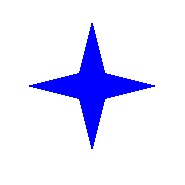
\includegraphics[width=3cm]{XXX2}
\\ 
\hline \BS{includegraphics}\AC{XXX1} &  \BS{includegraphics}\AC{XXX2}\\ 
\hline 
\end{tabular} 


\begin{minipage}{7cm}
\animategraphics[controls,loop,autoplay]{4}{XXX}{1}{2}  
\end{minipage}\hfill
\begin{minipage}{7cm}
\begin{tabular}{|l@{:}l|}
\hline \BSS{animategraphics} &  \\ 
\hline [ controls, & \TFRGB{boutons de contrôle}{Inserts control buttons} \\ 
\hline loop &  \TFRGB{en boucle}{animation restarts automatically}\\ 
\hline autoplay ] & \TFRGB{auto démarrage}{Start animation automatically } \\ 
\hline \AC{4} &  \TFRGB{4 fois par seconde}{4 frame per second}\\ 
\hline \AC{XXX} & \TFRGB{base du nom fichier}{file base name} \\ 
\hline \AC{1} & \TFRGB{numero de début}{number of the first frame} \\ 
\hline \AC{2} & \TFRGB{numero de fin}{number of the last frame} \\ 
\hline 
\end{tabular} 

\end{minipage}

%--------------------------------------------------------------
\subsection{Animateinline}




\begin{minipage}{5cm}
\begin{center}
\begin{animateinline}[ controls,loop,autoplay]{5}%

\begin{tikzpicture} 
\fill[blue] (45:2) -- (135:.5)-- (225:2)--(315:.5) -- cycle;
\fill[blue] (45:.5) -- (135:2)-- (225:.5)--(315:2) -- cycle;
 \end{tikzpicture}
\newframe%

\begin{tikzpicture} 
\fill[blue] (0:2) -- (90:.5)-- (180:2)--(270:.5) -- cycle;
\fill[blue] (0:.5) -- (90:2)-- (180:.5)--(270:2) -- cycle;
 \end{tikzpicture}
\end{animateinline}% 
\end{center}
\end{minipage}\hfill
\begin{minipage}{12cm}
\ESS{animateinline}[controls,loop,autoplay]\AC{5} \\

\emph{\% \TFRGB{première image}{first frame }}\\
\BS{begin\AC{tikzpicture} }
\BS{fill}[blue] (45:2) - - (135:.5)- - (225:2)- -(315:.5) - - cycle;
\BS{fill}[blue] (45:.5) - - (135:2)- - (225:.5)- -(315:2) - - cycle;
 \BS{end\AC{tikzpicture}}

\emph{\% \TFRGB{deuxième}{second frame }}\\
\BSS{newframe} \\
\BS{begin\AC{tikzpicture} } \\
\BS{fill}[blue] (0:2) - - (90:.5)- - (180:2)- -(270:.5) - - cycle; \\
\BS{fill}[blue] (0:.5) - - (90:2)- - (180:.5)- -(270:2) - - cycle; \\
 \BS{end\AC{tikzpicture}} \\
 \\
\BS{end\AC{animateinline}} \\
\end{minipage}




\subsection{Multiframe}

\begin{minipage}{5cm}
\begin{center}
\begin{animateinline}[poster=first, controls, palindrome,autoplay]{12}%
\multiframe{29}{iAngle=80+10,Rdim=2.0+-0.2}{
\begin{tikzpicture} 
\fill[blue] (\iAngle+45:\Rdim) -- (\iAngle+135:.5)-- (\iAngle+225:\Rdim)--(\iAngle+315:.5) -- cycle;
\fill[blue] (\iAngle+45:.5) -- (\iAngle+135:\Rdim)-- (\iAngle+225:.5)--(\iAngle+315:\Rdim) -- cycle;
 \end{tikzpicture}
%\end{pspicture} 
}%
\end{animateinline}%
\end{center}
\end{minipage}\hfill
\begin{minipage}{12cm}
\BS{begin}\AC{animateinline}[poster=first,controls, palindrome]\AC{12} \\
\BSS{multiframe}\AC{29}\AC{{\color{red} iAngle}=80+10, {\color{red} Rdim}=2.0+-0.2}\{ \\
\BS{begin\AC{tikzpicture} } \\
\BS{fill}[blue] (\BS{iAngle}+45:\BS{Rdim}) - - (\BS{iAngle}+135:.5)- - (\BS{iAngle}+225:\BS{Rdim})- -(\BS{iAngle}+315:.5) - - cycle; \\
\BS{fill}[blue] (\BS{iAngle}+45:.5) - - (\BS{iAngle}+135:\BS{Rdim})- - (\BS{iAngle}+225:.5)- -(\BS{iAngle}+315:\BS{Rdim}) - - cycle; \\
 \BS{end\AC{tikzpicture}}
\} \\
\BS{end}\AC{animateinline}%
\end{minipage}
\bigskip

\TFRGB{L'initiale de la variable définit son type}{The first  letter of the variable name determines his type }

\begin{tabular}{|c|l|}
\hline  entier &  initiale : i ou I \\ 
\hline  réelles &  initiale : n, N, r ou R \\ 
\hline  longueurs & initiale : d ou D \\ 
\hline 
\end{tabular} 



\bigskip

%---------------------------------------------------------------------
\begin{minipage}{5cm}

\begin{animateinline}[autoplay,loop]{12}%
\multiframe{24}{iAngle=0+15,icol=0+5}{\begin{tikzpicture}[rotate=90] %
  \draw[line width=0pt] (-2,-2) rectangle(6,2); %
  \draw  (0,0) node[fill=white,circle,rotate=\iAngle] {
\includegraphics[width=2cm]{LogoIUT}}  (0,0) circle (1);
   \draw (0,0) circle (1);
   \coordinate (abc) at (${sqrt(9-sin(\iAngle)*sin(\iAngle))+cos(\iAngle)}*(1,0)$) ;
   \coordinate (xyz) at (\iAngle:1);
   \draw[ultra thick] (0,0) --(xyz); 
   \draw[ultra thick] (xyz) -- (abc) ;
   \fill[color=blue!\icol] (abc)++(0.5,-1) rectangle (5,1) ;
   \draw[ultra thick] (abc) ++(0,-1) rectangle ++(.5,2) ;
   \draw[ultra thick]  (1.5,1) -- (5,1) -- (5,-1) -- (1.5,-1);
   \fill[red] (xyz) circle (4pt);
   \fill[red] (abc) circle (4pt); 
 \end{tikzpicture}}
\end{animateinline}
\end{minipage}\hfill
\begin{minipage}{12cm}
\BS{begin\AC{animateinline}}[autoplay,loop]\AC{12}\\
\BS{multiframe}\AC{24}\AC{iAngle=0+15,icol=0+5}\{\BS{begin\AC{tikzpicture}} \\
 \BS{draw}[line width=0pt] (-2,-3) rectangle(6,3); \\
  \BS{draw} (0,0) node[fill=white,circle,rotate=\BS{iAngle}] \\
   \AC{\BS{includegraphics}[width=2cm]\AC{LogoIUT}}  (0,0) circle (1);\\
   \BS{draw} (0,0) circle (1); \\
   \BS{coordinate} (abc) at (\$\AC{sqrt(9-sin(\BS{iAngle})*sin(\BS{iAngle}))+cos(\BS{iAngle})}*(1,0)\$) ; \\
   \BS{coordinate} (xyz) at (\BS{iAngle}:1); \\
   \BS{draw}[ultra thick] (0,0) - -(xyz); \\
   \BS{draw}[ultra thick] (xyz) - - (abc) ; \\
   \BS{fill}[color=blue{}!\BS{icol}] (abc)++(0.5,-1) rectangle (5,1) ; \\
   \BS{draw}[ultra thick] (abc) ++(0,-1) rectangle ++(.5,2) ; \\
   \BS{draw}[ultra thick]  (1.5,1) - - (5,1) - - (5,-1) - - (1.5,-1); \\
   \BS{fill}[red] (xyz) circle (4pt); \\
   \BS{fill}[red] (abc) circle (4pt); \\
 \BS{end\AC{tikzpicture}}\} \\
\BS{end\AC{animateinline}}

\end{minipage}
